\documentclass[10pt]{beamer}

%%%
% PREAMBLE FOR THIS DOC 
%%%
%https://tex.stackexchange.com/questions/68821/is-it-possible-to-create-a-latex-preamble-header
\usepackage{/Users/miw267/Repos/latex_preamble/beamer_preamble}



%%%
% COMMANDS SPECIFIC TO THIS DOC
%%%

% PROBABILISTIC GRAPHICAL MODELS (PGM's)
\newcommand{\parents}{\textbf{pa}}
\newcommand{\coparents}{\textbf{cp}}
\newcommand{\children}{\textbf{ch}}
\newcommand{\parent}{\text{pa}}
\newcommand{\coparent}{\text{cp}}
\newcommand{\child}{\text{ch}}

\usepackage{subcaption}



\agendatopic[what]{What is a graph?}
\agendatopic[history]{History: Bridge of K\text{\"o}nigsberg}
\agendatopic[examples]{Cool modern examples}
\agendatopic[theory]{Theory: A first peek}
\agendatopic[probability]{Probabilistic graphical models}
%%%
% DOCUMENT
%%%

\begin{document}



\title{11/16/2026: Graph Theory Fundamentals}
\author{CSCI 246: Discrete Structures}
\date{Textbook reference: Sec 47, Scheinerman}

\begin{frame}
    \titlepage 
\end{frame}


\begin{frame}
%\small
%\begin{mygreenbox}[title=Graded Quiz Pickup]
%Quizzes are in the front of the room, grouped into four bins (A-G, H-L, M-R, S-Z) by last name. The quizzes are upside down with your last name on the back. Come find yours before, during, or after class. Only turn the quiz over if it's yours.
%\end{mygreenbox} 
%\vfill 
%\begin{myredbox}[title=Friday's Problems Quiz]
%The problems quiz on Friday (04/02) will cover:
%\begin{itemize}
%\item Conditional Probability and Independence
%\item Random Variables
%\item Expectations	
%\end{itemize}
%
%\end{myredbox}
\vfill 

\begin{myredbox}[title=Announcement]
The reading for class on Wed 11/16 is changed to a section of the Lovacz textbook.\\
\\
After class, I will update the syllabus, make a Canvas announcement,  and provide the link.\\
\\
On Wednesday we'll start with an \alert{extra credit} question based on your reading.
\end{myredbox}
\vfill 
\begin{myyellowbox}[title=Today's Agenda]
\begin{itemize}
	\item Odds and Ends ($\approx$ 5 mins)
	\item Mini-lecture ($\approx$ 25 mins)
	\item Group exercises ($\approx$ 20 mins)
\end{itemize}


\end{myyellowbox}
\vfill 

\end{frame}



\agendaframe{what}


\begin{frame}{What is a graph?}

\begin{mygreenbox}[title=\text{Definition: Graph}]
A \textbf{graph} is a pair $G = (V, E)$, where
\begin{itemize}
\item $V$ is a set of \textbf{vertices} (also called nodes), and
\item $E$ is a set of \textbf{edges}, where each edge is a set of two vertices $\set{u, v}$.
\end{itemize}
\end{mygreenbox}

\vfill

\colorbox{yellow!30}{\textbf{Example.}}

\begin{columns}[c,onlytextwidth]
\begin{column}{0.4\textwidth}
\centering
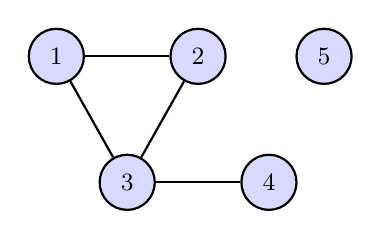
\begin{tikzpicture}[
    vertex/.style={circle, draw, thick, fill=blue!15, minimum size=7mm, font=\small},
    every edge/.style={draw, thick}]
  \node[vertex] (1) at (0,1.6) {1};
  \node[vertex] (2) at (1.8,1.6) {2};
  \node[vertex] (3) at (0.9,0) {3};
  \node[vertex] (4) at (2.7,0) {4};
  \node[vertex] (5) at (3.4,1.6) {5};
  \path (1) edge (2)
        (1) edge (3)
        (2) edge (3)
        (3) edge (4);
\end{tikzpicture}
\end{column}
\begin{column}{0.56\textwidth}

$V = \set{1, 2, 3, 4, 5}$

\vspace{8pt}
$E = \big\{ \set{1,2}, \set{1,3}, \set{2,3}, \set{3,4} \big\}$

\vspace{8pt}
%{\small Vertex 5 has no edges, but it is still a vertex of $G$.}
\end{column}
\end{columns}

\pause 
\scriptsize 
\colorbox{red!30}{\textbf{Terminology.}}
\begin{itemize}
\item Two nodes with an edge between are \textbf{adjacent}. \pause 
\item The \textbf{degree} of a node is the number of edges with that node as an endpoint.
\end{itemize}




\vfill
\end{frame}



\begin{frame}{One graph, many drawings}

Here are three drawings of the graph $G = (V,E)$ with
\[ V = \set{1,2,3,4,5}, \qquad E = \big\{ \set{1,2}, \set{1,3}, \set{2,3}, \set{3,4} \big\}. \]

\vfill

\tikzset{
  vertex/.style={circle, draw, thick, fill=blue!15, minimum size=6mm, inner sep=0pt, font=\small},
  every edge/.style={draw, thick}}
\begin{columns}[c,onlytextwidth]
\begin{column}{0.32\textwidth}
\centering
\begin{tikzpicture}
  \node[vertex] (1) at (0,1.4) {1};
  \node[vertex] (2) at (1.5,1.4) {2};
  \node[vertex] (3) at (0.75,0) {3};
  \node[vertex] (4) at (2.25,0) {4};
  \node[vertex] (5) at (2.8,1.4) {5};
  \path (1) edge (2) (1) edge (3) (2) edge (3) (3) edge (4);
\end{tikzpicture}
\end{column}
\begin{column}{0.32\textwidth}
\centering
\onslide<2->{%
\begin{tikzpicture}
  \node[vertex] (3) at (1.2,0.7) {3};
  \node[vertex] (4) at (0,0.7) {4};
  \node[vertex] (1) at (2.2,1.5) {1};
  \node[vertex] (2) at (2.2,-0.1) {2};
  \node[vertex] (5) at (0.4,-0.1) {5};
  \path (1) edge (2) (1) edge (3) (2) edge (3) (3) edge (4);
\end{tikzpicture}}
\end{column}
\begin{column}{0.32\textwidth}
\centering
\onslide<3->{%
\begin{tikzpicture}
  \node[vertex] (1) at (0,0) {1};
  \node[vertex] (2) at (2.4,1.4) {2};
  \node[vertex] (3) at (2.4,0) {3};
  \node[vertex] (4) at (0,1.4) {4};
  \node[vertex] (5) at (1.2,-0.6) {5};
  \path (1) edge[bend left=60] (2) (1) edge (3) (2) edge (3) (3) edge (4);
\end{tikzpicture}}
\end{column}
\end{columns}

\vfill
\onslide<4->{%
\begin{mygreenbox}[title=\text{Key idea}]
A graph is determined only by \textbf{which vertices are adjacent to which}.  The positions of the vertices, the lengths and shapes of the edges, and whether edges cross in the drawing do not matter.
\end{mygreenbox}}
\end{frame}


\agendaframe{history}



\begin{frame}{Graphs as abstractions: The Bridge of K\text{\"o}nigsberg.}

\small 

\begin{minipage}{.47\textwidth}

\onslide+<1->\begin{figure}
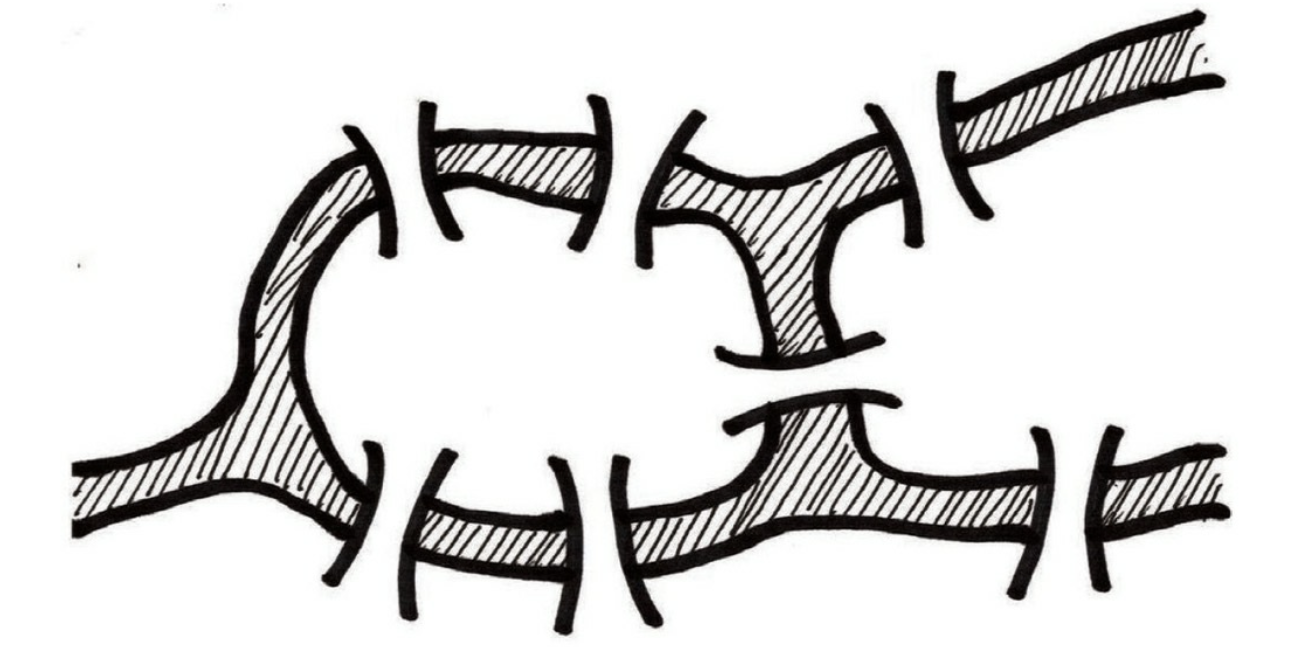
\includegraphics[width=.8\linewidth]{images/konigsberg.png}	
\caption{Bridge of K\text{\"o}nigsberg.}
\end{figure}
\end{minipage} %
\hfill 
\begin{minipage}{.47\textwidth}
\onslide+<3->\begin{figure}
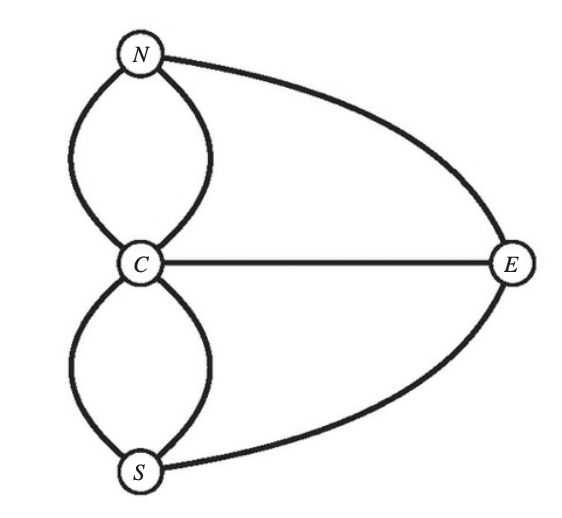
\includegraphics[width=.8\linewidth]{images/konigsberg_graph.png}
\caption{Graph representation}	
\end{figure}

\end{minipage} %

\vfill 
\onslide+<1-> \colorbox{green!30}{\textbf{Claim.}}  There was a pub on the center
island, with challenges and late-night attempts to “walk the bridges,” to make a tour of the town crossing every bridge exactly once. Despite the accompanying boasts, rarely reproducible in the sober morning, this was a difficult task.  Most who attempted found that they had missed a bridge or that they crossed a bridge twice.
\vfill 
\onslide+<2-> \colorbox{red!30}{\textbf{Question.}} Can you find a tour of the town that traverses each of the seven bridges exactly once? \hfill \onslide+<4-> \href{https://www.youtube.com/watch?v=C7YrMRdLkqo}{\underline{\blue{Click here for short video.}}}
\end{frame}



\agendaframe{examples}


\begin{frame}{High school romantic/sexual network}

\begin{center}
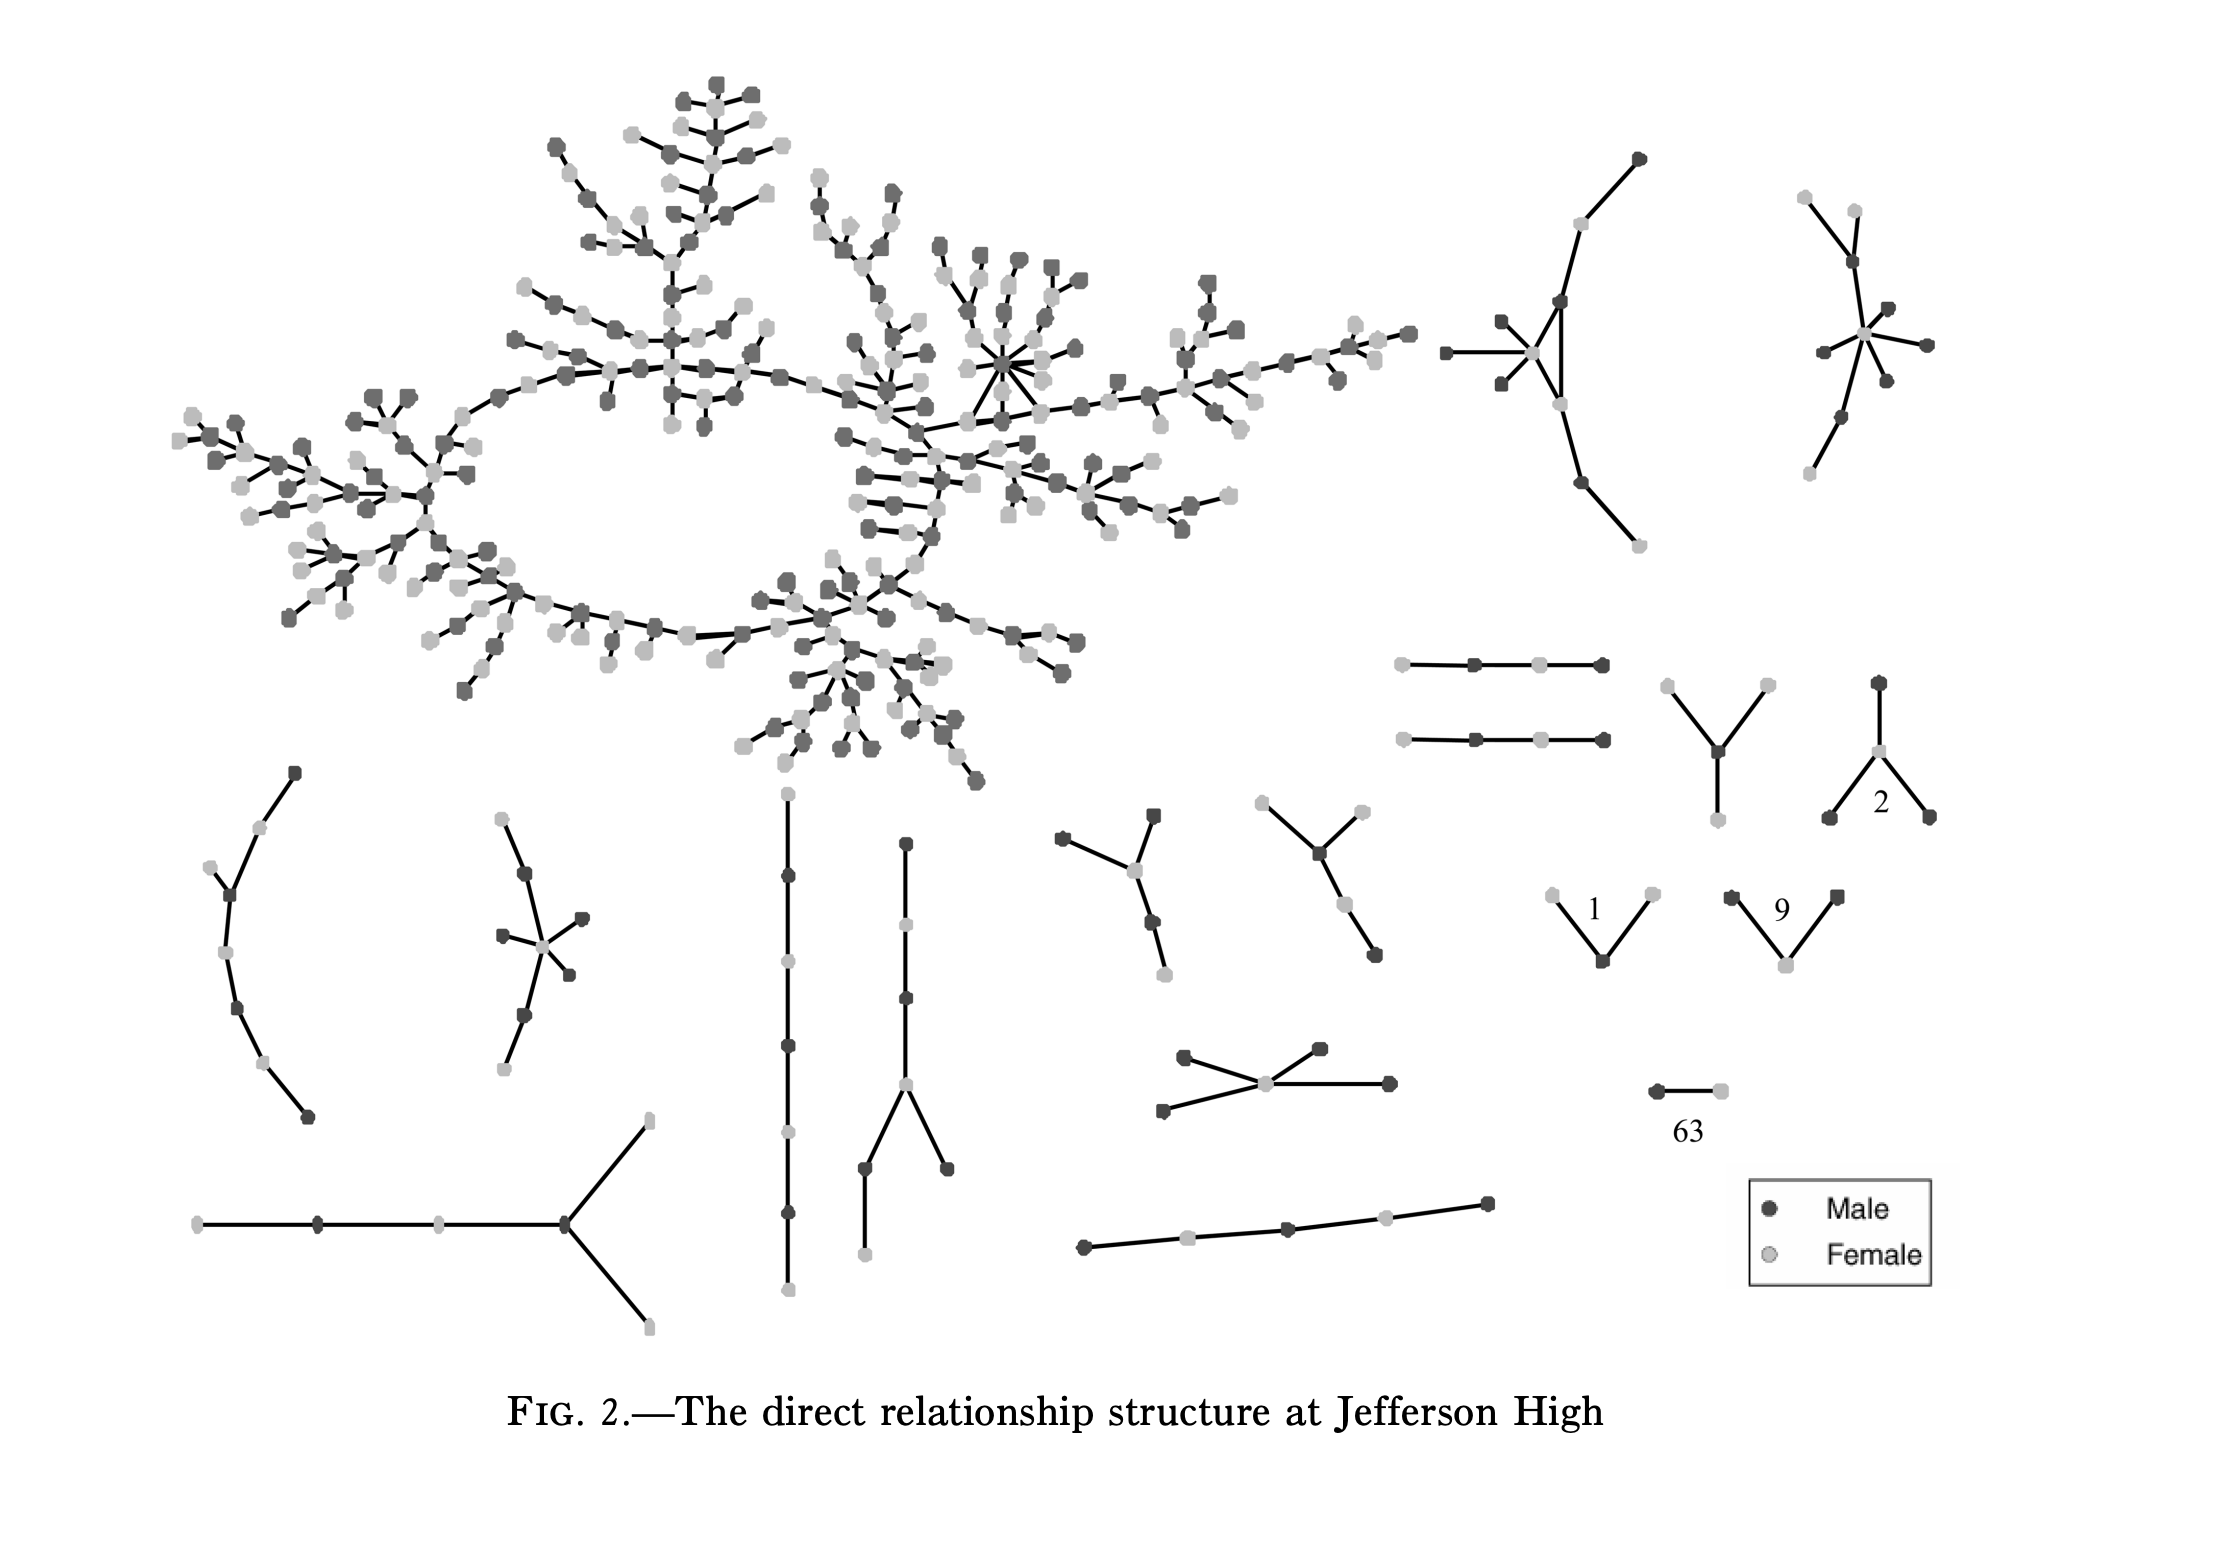
\includegraphics[height=0.64\textheight]{images/affection.png}
\end{center}

\scriptsize 
\colorbox{red!30}{\textbf{Observations?}} \pause 
\begin{itemize}
\item The graph decomposes into multiple \textbf{components}, including one very large one. \pause 
\item \qq{The size of the large component of connected nodes identifies the worst case scenario for potential disease diffusion within the population.}
\end{itemize}



\citebottom{Bearman, P. S., Moody, J., \& Stovel, K. (2004). Chains of affection: The structure of adolescent romantic and sexual networks. American journal of sociology, 110(1), 44-91.}
\end{frame}


\begin{frame}{Community structure of political blogs}


\only<1-2>{
\begin{center}
\blue{Liberal} and \red{conservative} blogs have few links between them. 
\end{center}
}

\only<1-2>{
\begin{center}
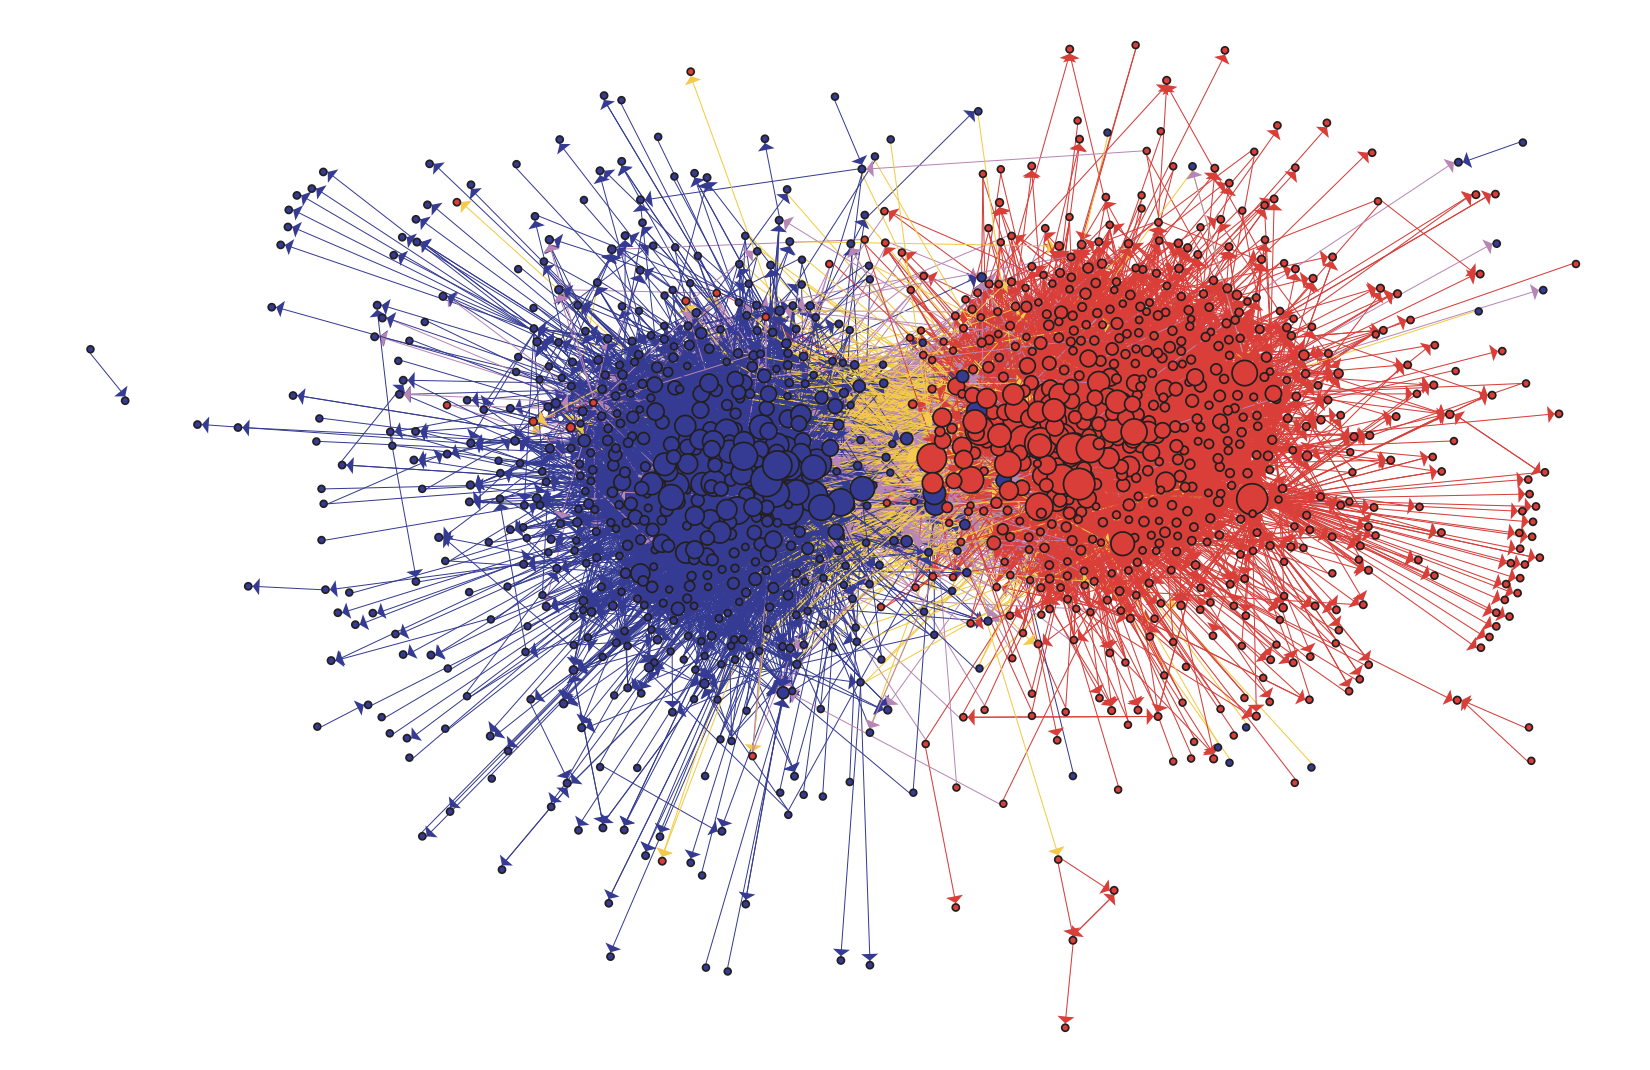
\includegraphics[height=0.5\textheight]{images/divided1.png}

\vspace{.05cm}
\only<2>{\colorbox{yellow!30}{\textbf{Terminology.}}  The network has two \textbf{communities} (or \textbf{clusters}): groups of nodes with many edges inside and few edges between.}
\end{center}
}


\only<3->{
\begin{center}
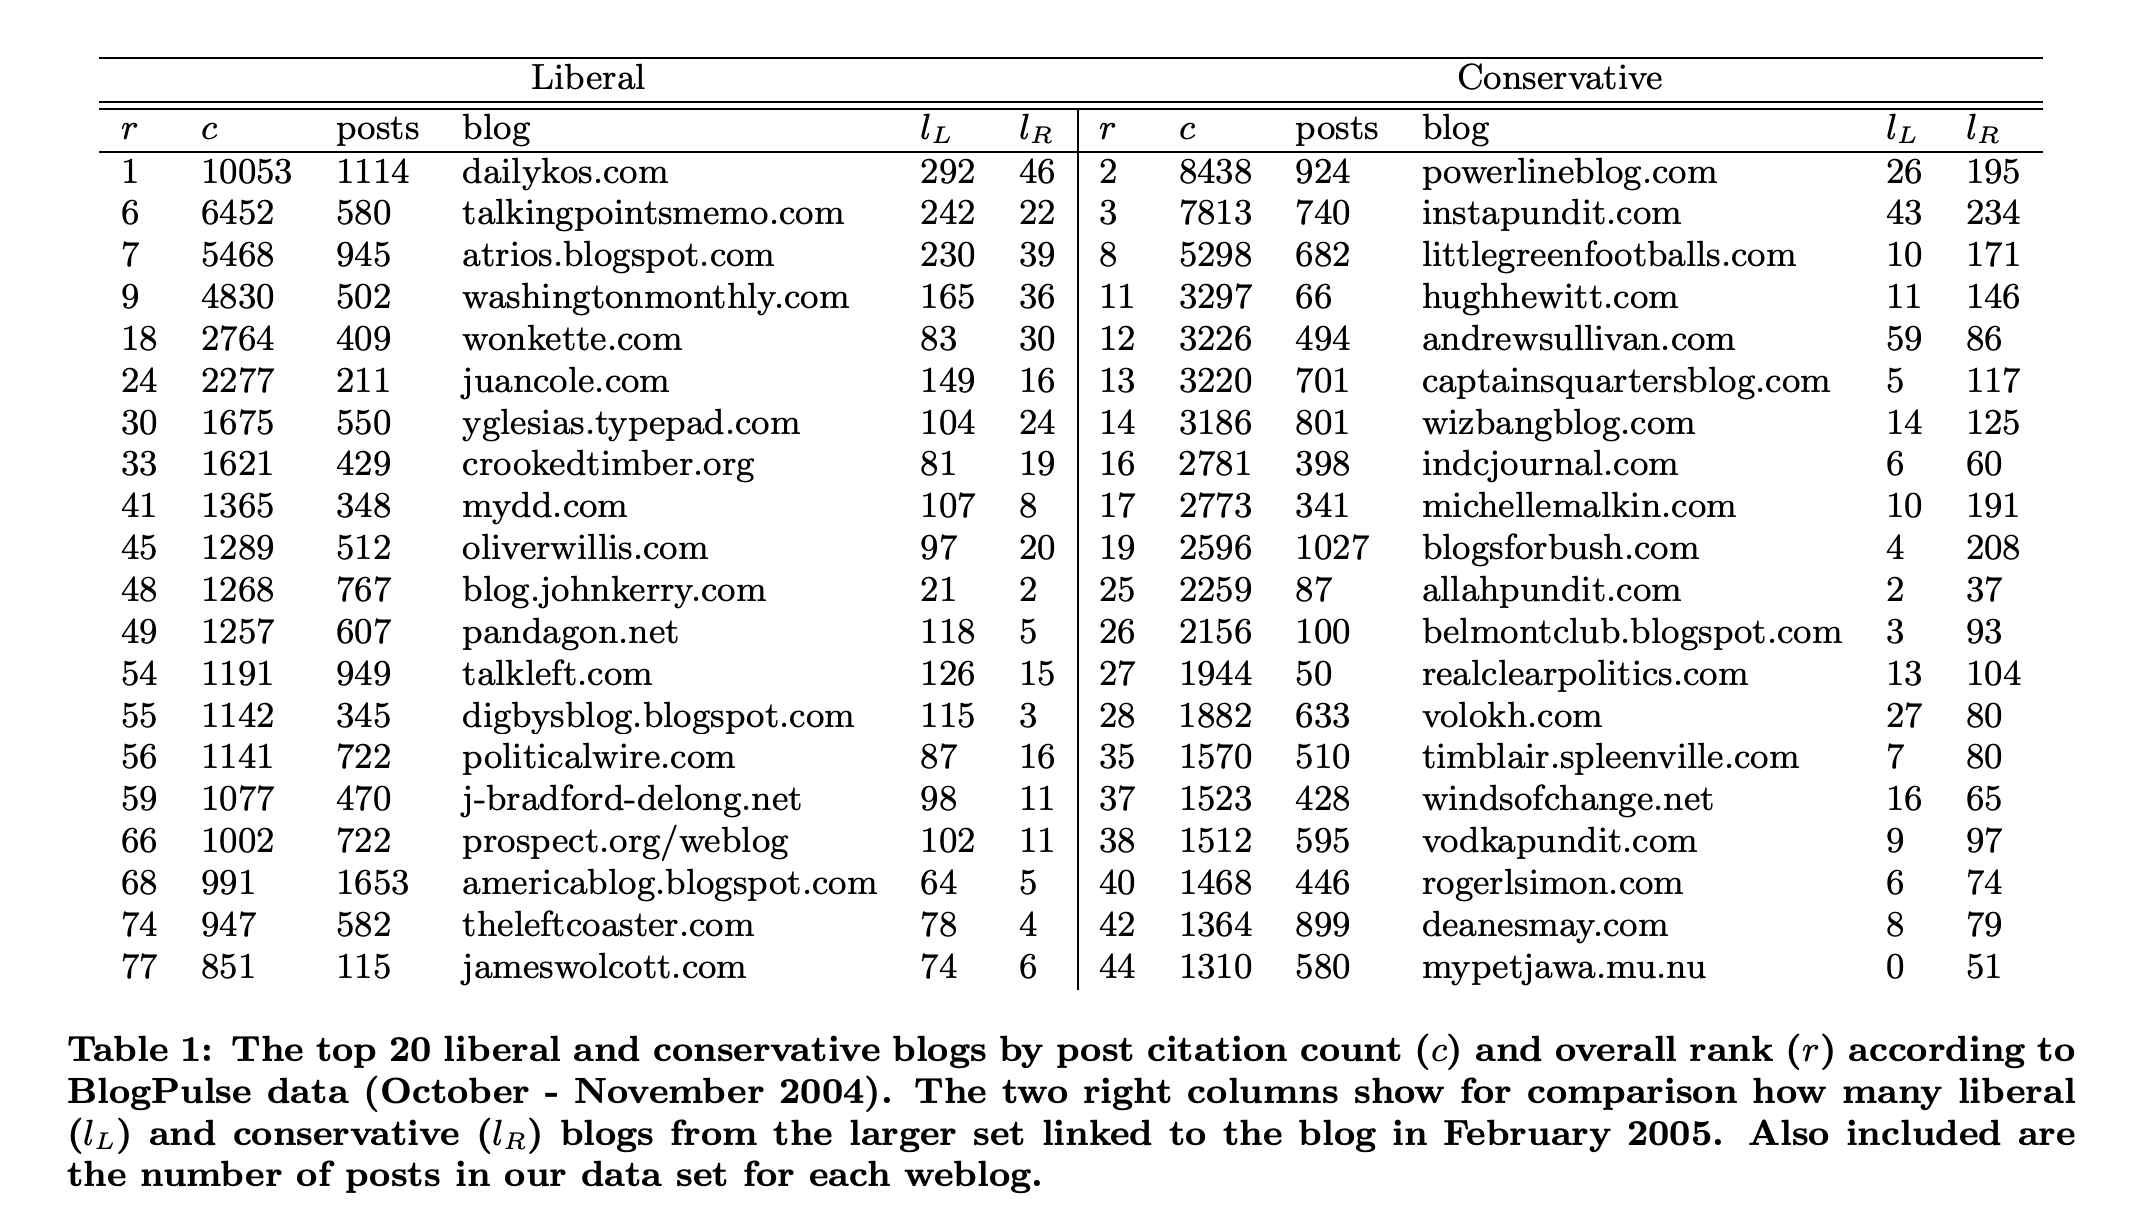
\includegraphics[height=0.5\textheight]{images/divided2.png}
\end{center}
}



\citebottom{
Adamic, L. A., \& Glance, N. (2005, August). The political blogosphere and the 2004 US election: divided they blog. In Proceedings of the 3rd international workshop on Link discovery (pp. 36-43).
}
\end{frame}



\begin{frame}{Zachary's Karate Club}

\scriptsize 
An edge between two members means they socialized outside the club’s regular classes. 

\begin{center}
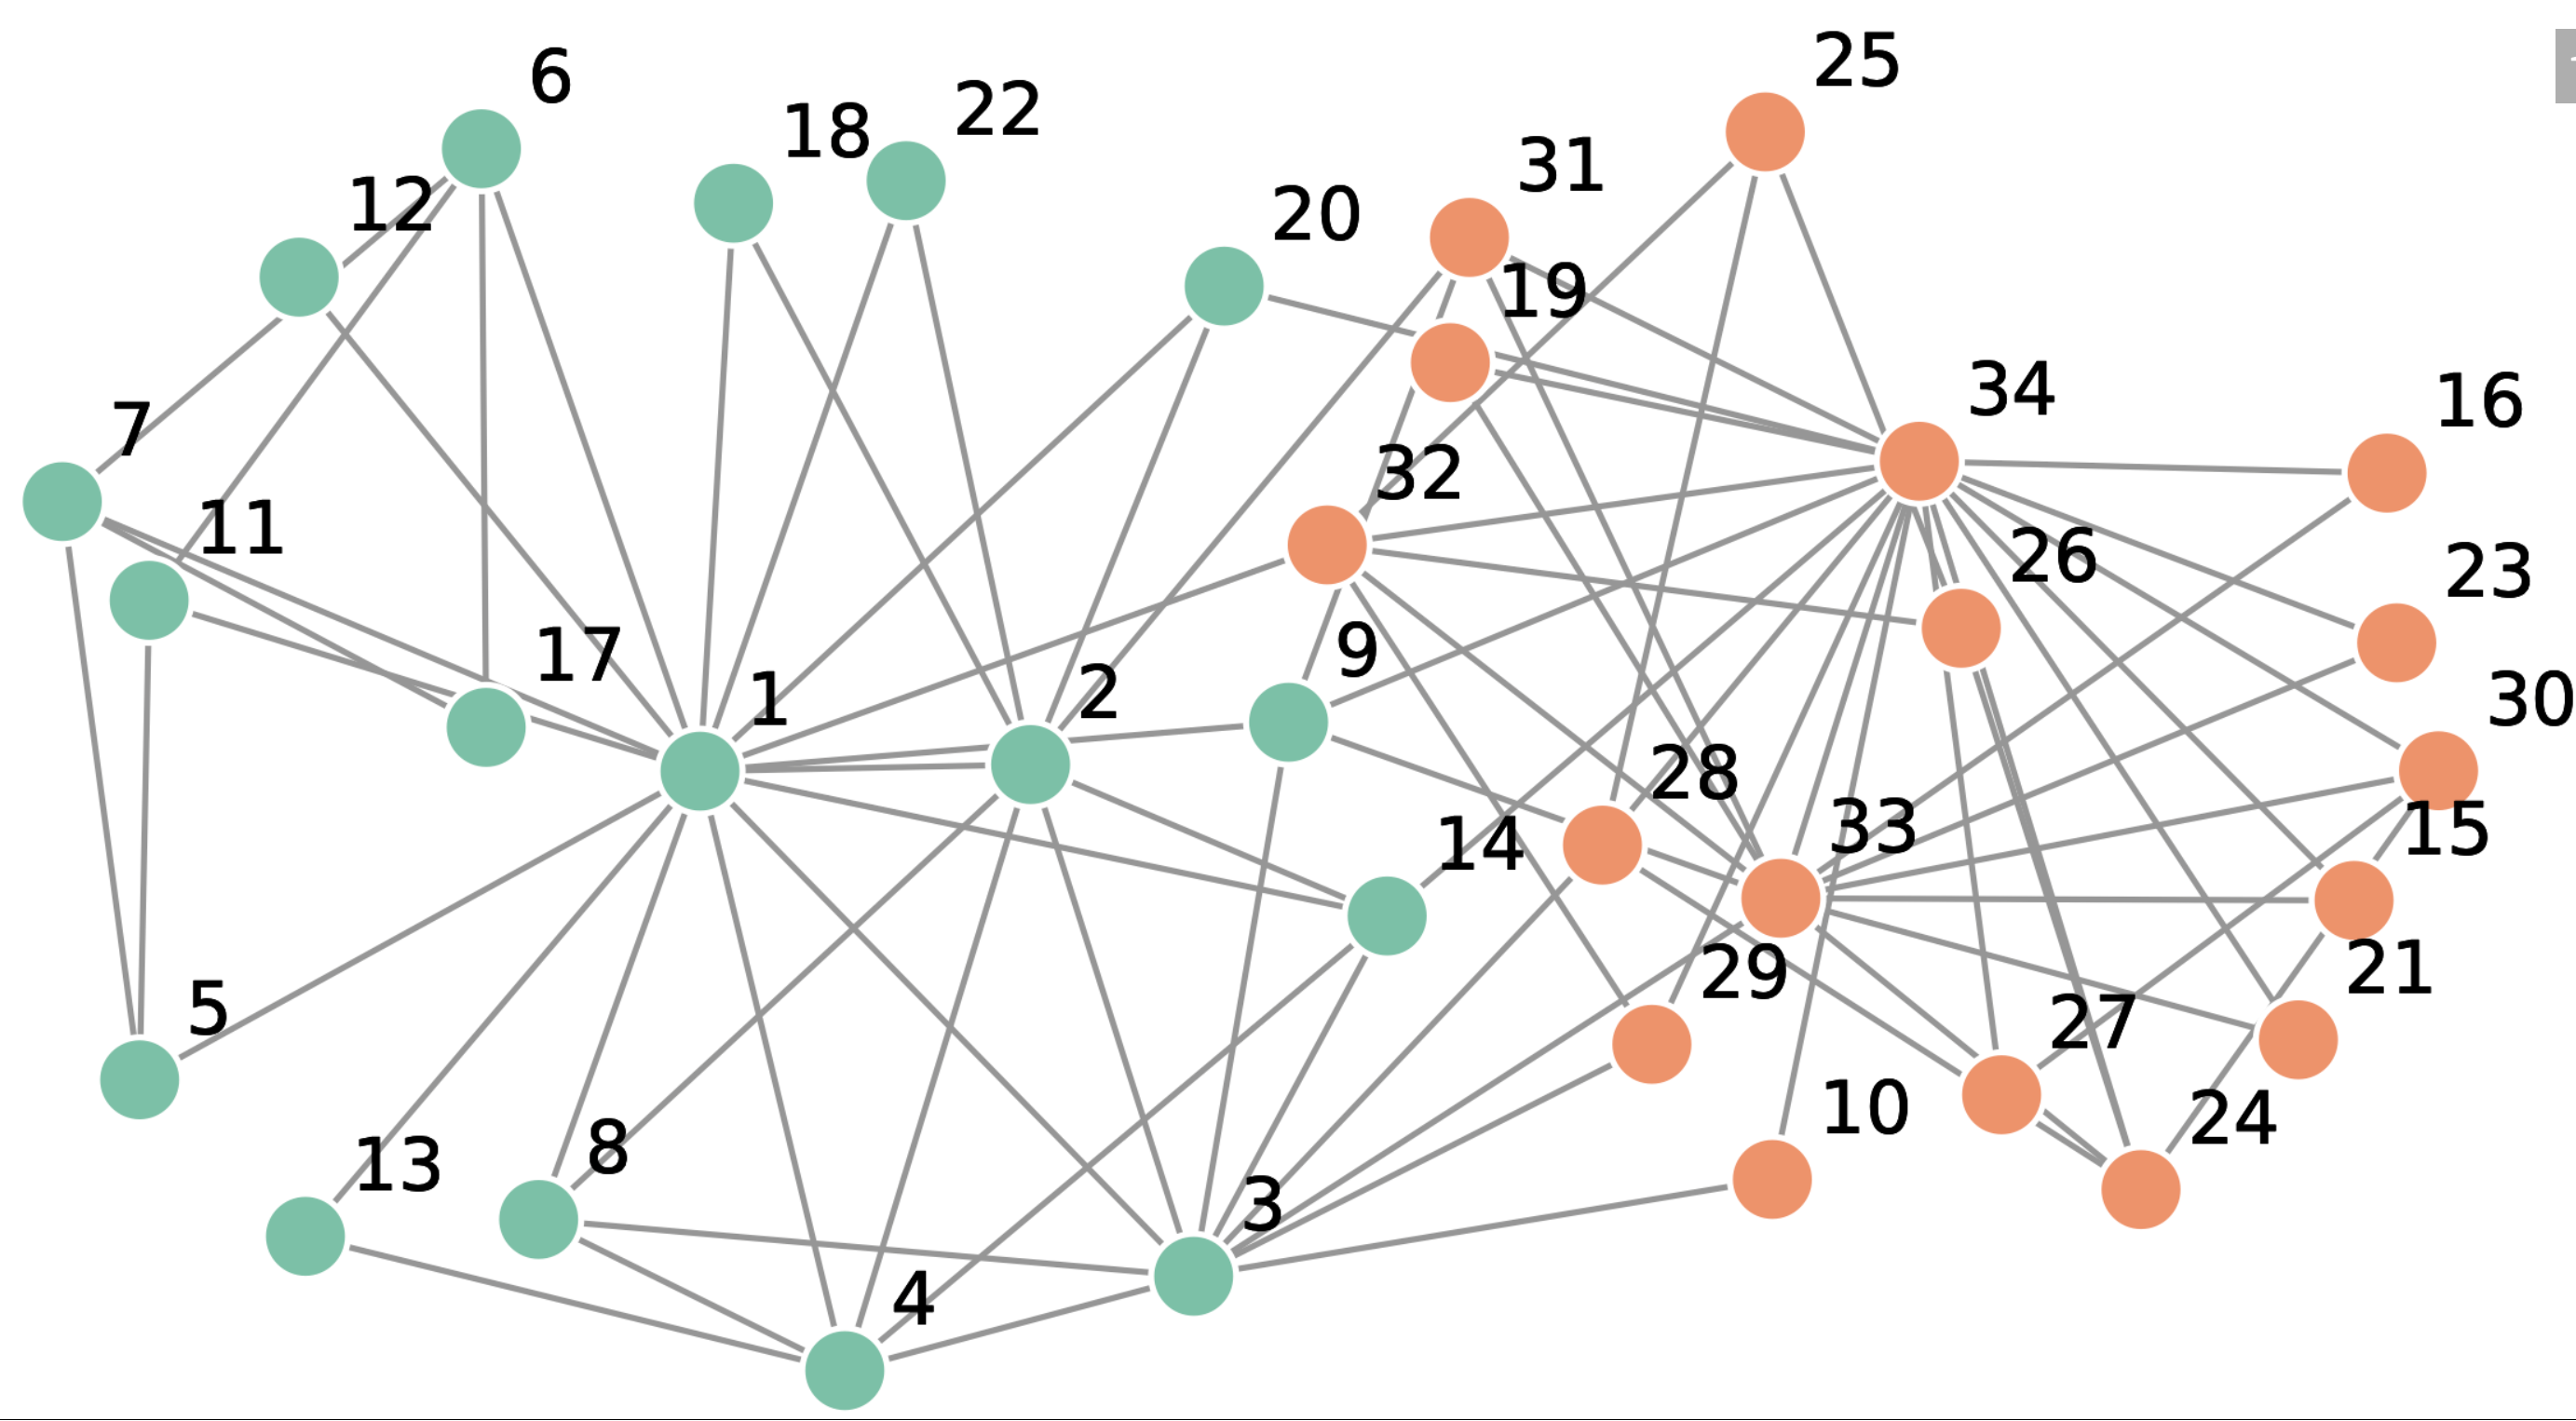
\includegraphics[height=0.5\textheight]{images/karate.png}
\end{center}

\pause 

\colorbox{yellow!30}{\textbf{Why is this graph famous?}} \pause   During the study, a conflict between the club’s instructor (\qq{Mr. Hi}) and its president (\qq{John A.}) split the club in two. 
\pause 

A \qq{minimum cut} through the friendship graph, separating the two leaders with as few edges as possible, predicted  which members went with which side -- with only \textbf{one} exception! 
\pause 
\vfill 
So the friendship network alone, drawn before the split, \alert{predicted} the split!
	
\end{frame}

\begin{frame}{Functional Brain Region Connectivity In Depression}

Depression is associated with changes (\red{increase} vs. \blue{decrease}) in the functional connectivity of brain regions.

\begin{columns}[c,onlytextwidth]

\begin{column}{0.45\textwidth}
\centering
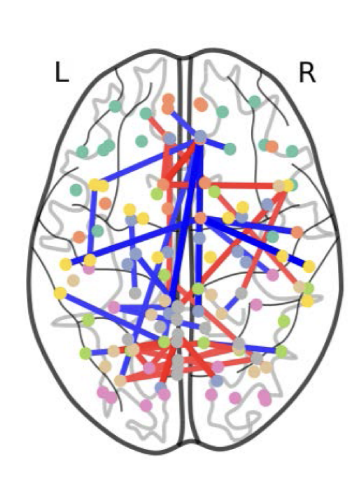
\includegraphics[height=0.7\textheight]{images/depression_1.png}
\end{column}

\begin{column}{0.45\textwidth}
\centering
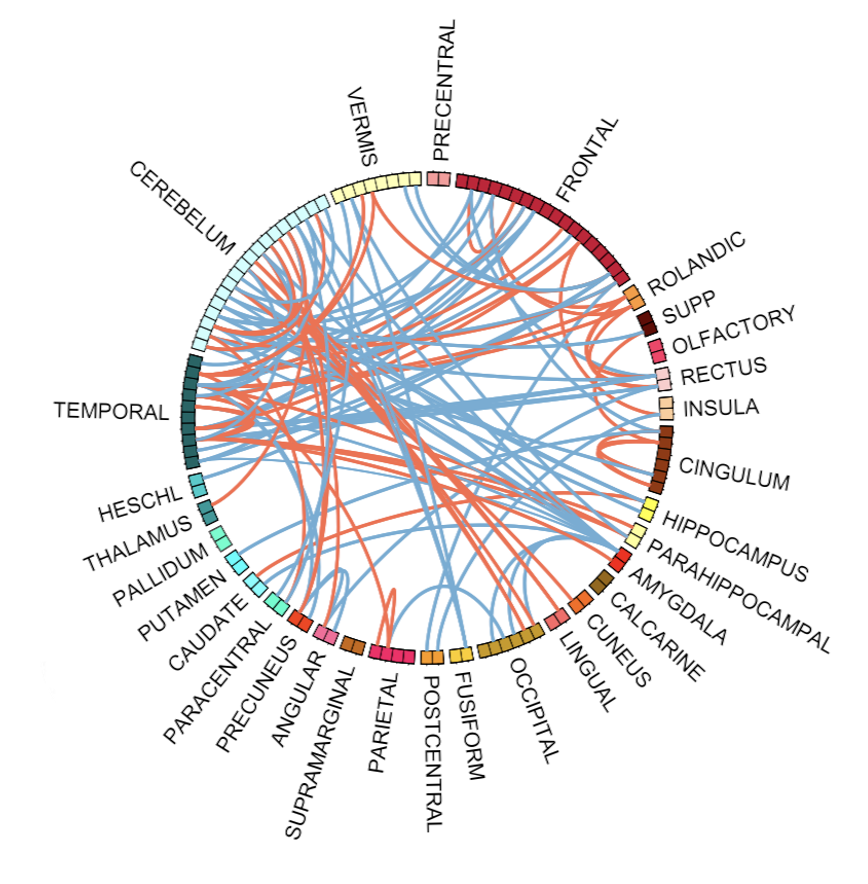
\includegraphics[height=0.7\textheight]{images/depression_2.png}
\end{column}
\begin{column}{0.05\textwidth}
\end{column}


\end{columns}

\citebottom{Noman, F., Ting, C. M., Kang, H., Phan, R. C. W., \& Ombao, H. (2024). Graph autoencoders for embedding learning in brain networks and major depressive disorder identification. IEEE journal of biomedical and health informatics, 28(3), 1644-1655.}
\end{frame}






\agendaframe{theory}



\begin{frame}
\footnotesize 
\begin{myredbox}[title=Reading Quiz (Graph Theory Fundamentals)]
 Let $G=(V,E)$.  The sum of the degree of vertices in G is \textit{how many} times the number of edges? That is, if we write
\[ \sum_{v \in V} \deg(v) = C|E|, \]
What is $C$? Give a brief explanation for your answer.

\end{myredbox}
\vfill 
\pause 

\begin{mygreenbox}[title=\text{Theorem (Handshake Lemma)}]
For any graph $G = (V,E)$, \qquad $\displaystyle \sum_{v \in V} \deg(v) = 2\,|E|$.
\end{mygreenbox}

\vfill
\pause
\colorbox{yellow!30}{\textbf{Example.}}

\begin{columns}[c,onlytextwidth]
\begin{column}{0.45\textwidth}
\centering
\begin{tikzpicture}[
    vertex/.style={circle, draw, thick, fill=blue!15, minimum size=7mm, font=\small},
    deg/.style={font=\footnotesize, text=red!70!black},
    every edge/.style={draw, thick}]
  \node[vertex] (1) at (0,1.6) {1};
  \node[vertex] (2) at (1.8,1.6) {2};
  \node[vertex] (3) at (0.9,0) {3};
  \node[vertex] (4) at (2.7,0) {4};
  \node[vertex] (5) at (3.4,1.6) {5};
  \path (1) edge (2) (1) edge (3) (2) edge (3) (3) edge (4);
  \onslide<3->{
  \node[deg, above=1pt of 1] {deg 2};
  \node[deg, above=1pt of 2] {deg 2};
  \node[deg, below=1pt of 3] {deg 3};
  \node[deg, below=1pt of 4] {deg 1};
  \node[deg, above=1pt of 5] {deg 0};
  }
\end{tikzpicture}
\end{column}
\begin{column}{0.51\textwidth}
\onslide<4->{Sum of degrees: $2 + 2 + 3 + 1 + 0 = 8$}

\vspace{5pt}
\onslide<5->{Number of edges: $|E| = 4$, \quad and $8 = 2 \cdot 4$. \checkmark}

\vspace{5pt}
%\onslide<6->{\colorbox{green!30}{\textbf{Why?}} Each edge has two ends, and each end adds 1 to the degree of a vertex.  So summing the degrees counts every edge exactly twice.}
\onslide<6->{\colorbox{green!30}{\textbf{Why?}} Each edge has two ends.  So summing the degrees counts every edge exactly twice.}
\end{column}
\end{columns}

\end{frame}



\begin{frame}{Why is the Handshake Lemma Useful?}

Some examples:
\begin{enumerate}
	\item \textbf{Proving that some graphs can’t exist.} Can 7 people each shake hands with exactly 3 others? No: the degrees would sum to 7 × 3 = 21, which is odd. \pause 
	\item \textbf{Average degree.} The average degree is $\frac{2|E|}{|V|}$, which is how the \qq{average number of friends} on a social network is computed from the number of friendships. \pause 
	\item \textbf{Analyzing algorithms.} When an algorithm visits every vertex and loops over its neighbors, the total work in those loops is the sum of the degrees, which is $2|E|$. That’s why graph search runs in $O(|V| + |E|)$ time.
\end{enumerate}
\end{frame}

\agendaframe{probability}


\begin{frame}{Probabilistic Graphical Models: The Idea}
\setlength{\abovedisplayskip}{3pt}
\setlength{\belowdisplayskip}{3pt}

\only<1-4>{By the \textbf{chain rule}, any joint distribution can be factored as follows, corresponding to the \textit{complete} graph:}%
\only<5>{In many problems, some variables can be dropped from the conditioning set.  Correspondingly, we can drop some edges from the graph.}%
\only<6->{The strategy of representing probability distributions as graphs is called \textbf{probabilistic graphical models}.}

{\small
\only<1-4>{%
\begin{align*}
p(\+x) &= p(x_1) \, p(x_2 \cond x_1) \, p(x_3 \cond x_1, x_2) \, p(x_4 \cond x_1, x_2, x_3) \\
&\quad \times p(x_5 \cond x_1, x_2, x_3, x_4) \, p(x_6 \cond x_1, x_2, x_3, x_4, x_5)
\end{align*}}%
\only<5>{%
\begin{align*}
p(\+x) &= p(x_1) \, p(x_2 \cond x_1) \, p(x_3 \cond x_1, \cancel{x_2}) \, p(x_4 \cond \cancel{x_1}, x_2, \cancel{x_3}) \\
&\quad \times p(x_5 \cond \cancel{x_1}, \cancel{x_2}, x_3, \cancel{x_4}) \, p(x_6 \cond \cancel{x_1}, x_2, \cancel{x_3}, \cancel{x_4}, x_5)
\end{align*}}%
\only<6-7>{%
\begin{align*}
\setlength{\fboxsep}{1.5pt}
p(\+x) &= p(x_1) \, p(x_2 \cond \colorbox{blue!20}{$x_1$}) \, p(x_3 \cond \colorbox{blue!20}{$x_1$}) \, p(x_4 \cond \colorbox{blue!20}{$x_2$}) \, p(x_5 \cond \colorbox{blue!20}{$x_3$}) \, p(x_6 \cond \colorbox{blue!20}{$x_2, x_5$})
%p(\+x) &= p(x_1) \, p(x_2 \cond \blue{x_1}) \, p(x_3 \cond \blue{x_1}) \, p(x_4 \cond \blue{x_2}) \, p(x_5 \cond \blue{x_3}) \, p(x_6 \cond \blue{x_2, x_5})
\end{align*}}
\only<8->{%
\begin{align*}
p(\+x) &= p(x_1) \, p(x_2 \cond x_1) \, p(x_3 \cond x_1) \, p(x_4 \cond x_2) \, p(x_5 \cond x_3) \, p(x_6 \cond x_2, x_5)
\end{align*}}
}

\begin{figure}[H]
  \centering
  \scalebox{0.72}{%
  \tikz{ %
    % vertices on a regular hexagon, so the complete graph's crossings are symmetric
    \node[latent] (x1) at (180:1.8) {$x_1$} ; %
    \node[latent] (x2) at (120:1.8) {$x_2$} ; %
    \node[latent] (x4) at (60:1.8)  {$x_4$} ; %
    \node[latent] (x6) at (0:1.8)   {$x_6$} ; %
    \node[latent] (x5) at (-60:1.8) {$x_5$} ; %
    \node[latent] (x3) at (-120:1.8) {$x_3$} ; %
    % edges of the example Bayesian network
    \edge{x1}{x2};
    \edge{x1}{x3};
    \edge{x2}{x4};
    \edge{x2}{x6};
    \edge{x3}{x5};
    \edge{x5}{x6};
    % extra edges of the complete graph (chain rule), shown only on the first reveal
    \only<1-4>{
    \begin{scope}[->, >={triangle 45}, gray]
      \draw (x1) -- (x4);
      \draw (x1) -- (x5);
      \draw (x1) -- (x6);
      \draw (x2) -- (x3);
      \draw (x2) -- (x5);
      \draw (x3) -- (x4);
      \draw (x3) -- (x6);
      \draw (x4) -- (x5);
      \draw (x4) -- (x6);
    \end{scope}}
  }}

\only<1-4>{\caption{The complete graph implied by the chain rule}}%
\par
\begin{minipage}[t][1.1cm]{\linewidth}
\raggedright\small
\only<2-3>{\alert{What is a complete graph?}}
\only<3>{A \textbf{complete graph} is a graph in which every pair of distinct vertices is joined by an edge.}
\only<4-5>{\colorbox{red!30}{\textbf{Hot tip.}} Think of these factorizations in terms of steps you can take to \underline{simulate} data from the model.}
\only<6-7>{\colorbox{blue!30}{\textbf{Terminology.}} The variables in the conditioning set of $X_i$ are called the \blue{parents} of $X_i$.} \only<7>{The parents of $X_i$ are the variables whose edges point into $X_i$.}
\only<8-9>{\colorbox{green!30}{\textbf{Key Point.}} These graphs capture dependence/independence relationships between the variables.} \only<9>{However, there are some nuances!}
\end{minipage}


%\only<5->{\caption{An example Bayesian network}}
\label{fig:example_bayesian_network}
\end{figure}




\end{frame}




\begin{frame}[t]{Conditional vs. marginal independence}

\small 

\colorbox{green!30}{\textbf{Key point.}} Whether two variables are dependent can depend on whether a \textbf{third} variable is observed! \only<2->{\alert{Any examples?}}

\vspace{0.3cm}

\begin{columns}[T]
\begin{column}{0.70\textwidth}
\footnotesize
\onslide<3->{\colorbox{blue!30}{\textbf{Example.}}} %Consider the random variables: $I = \texttt{ice cream sales}$, $D = \texttt{drownings}$,  $C = \texttt{calendar date}$.}

\vspace{0.2cm}
\begin{itemize}\setlength{\itemsep}{3pt}
	\item<4-> Oddly, the \texttt{number of ice cream sales} $I$ and \texttt{number of drownings} $D$ are \alert{dependent} (positively correlated). \only<8->{$\bluemathbox{P(D \mid I) \neq P(D)}$}
	\item<5-> Why? \only<6>{Because both go up in the summer (or on the weekends).}
	\item<7-> A third variable, the \texttt{calendar date} $C$, explains away the dependence.
	\only<8->{So $D$ and $I$ are \alert{conditionally independent} (conditional on $C$).} \only<10->{$\bluemathbox{P(D \mid I, C) = P(D \mid C)}.$}
\end{itemize}
\end{column}
\begin{column}{0.27\textwidth}
\centering
\onslide<3->{
\includegraphics[width=.5\linewidth]{images/ice_cream}\\[1pt]{\scriptsize You live on the beach}}

\vspace{0.3cm}
\onslide<12->{%
\tikzset{
  cnode/.style = {latent, minimum size=0.9cm, line width=1.0pt, font=\large},
  cedge/.style = {->, >=latex, line width=1.0pt},
}
\resizebox{0.5\linewidth}{!}{%
  \begin{tikzpicture}
    \node[cnode] (x) at (-1, -2)  {$I$};
    \node[cnode] (y) at ( 1, -2)  {$D$};
    \alt<13>{\node[cnode, fill=gray!40] (z) at ( 0,0) {$C$};}{\node[cnode] (z) at ( 0,0) {$C$};}
    \draw[cedge] (z) -- (x);
    \draw[cedge] (z) -- (y);
  \end{tikzpicture}%
  }}
\end{column}
\end{columns}

\vfill
\only<11>{
\colorbox{red!30}{\textbf{Terminology.}} $I$ and $D$ are \textbf{marginally} dependent but \textbf{conditionally} independent (given $C$).
}

\only<12->{
\colorbox{yellow!30}{\textbf{Graphical View.}} The graph is drawn above.  $I$ and $D$ are dependent unless we observe $C$.
}


\end{frame}

\begin{frame}[t]{Conditional vs. marginal independence: Another Example}

\small 

\colorbox{green!30}{\textbf{Key point.}} Whether two variables are dependent can depend on whether a \textbf{third} variable is observed! %\only<2->{\alert{Any examples?}}

\vspace{0.3cm}

\begin{columns}[T]
\begin{column}{0.70\textwidth}
\footnotesize
\onslide<2->{\colorbox{blue!30}{\textbf{Example.}} Consider the binary random variables: $E = \texttt{earthquake}$, $B = \texttt{burglary}$,  $C = \texttt{car alarm}$.}

\vspace{0.2cm}
\begin{itemize}\setlength{\itemsep}{3pt}
	\item<3-> A priori, in S.F., earthquakes $E$ and burglaries $B$ are (approximately) \alert{independent}. \only<6->{$\bluemathbox{P(E \mid B=1) = P(E)}$}
	\item<4-> Now your car alarm $C$ goes off.  Given that, the probability of $E$ or $B$ rises. 
	\only<5->{  But if you hear there was an earthquake, the probability of a burglary goes back down, since the earthquake \alert{explains away} the burglary.}  \only<7->{So $E$ and $B$ are \alert{conditionally dependent}.} \only<7->{$\bluemathbox{P(E \mid C=1, B=1) \neq P(E \mid C=1)}$}
\end{itemize}
\end{column}
\begin{column}{0.27\textwidth}
\centering
%\onslide<3->{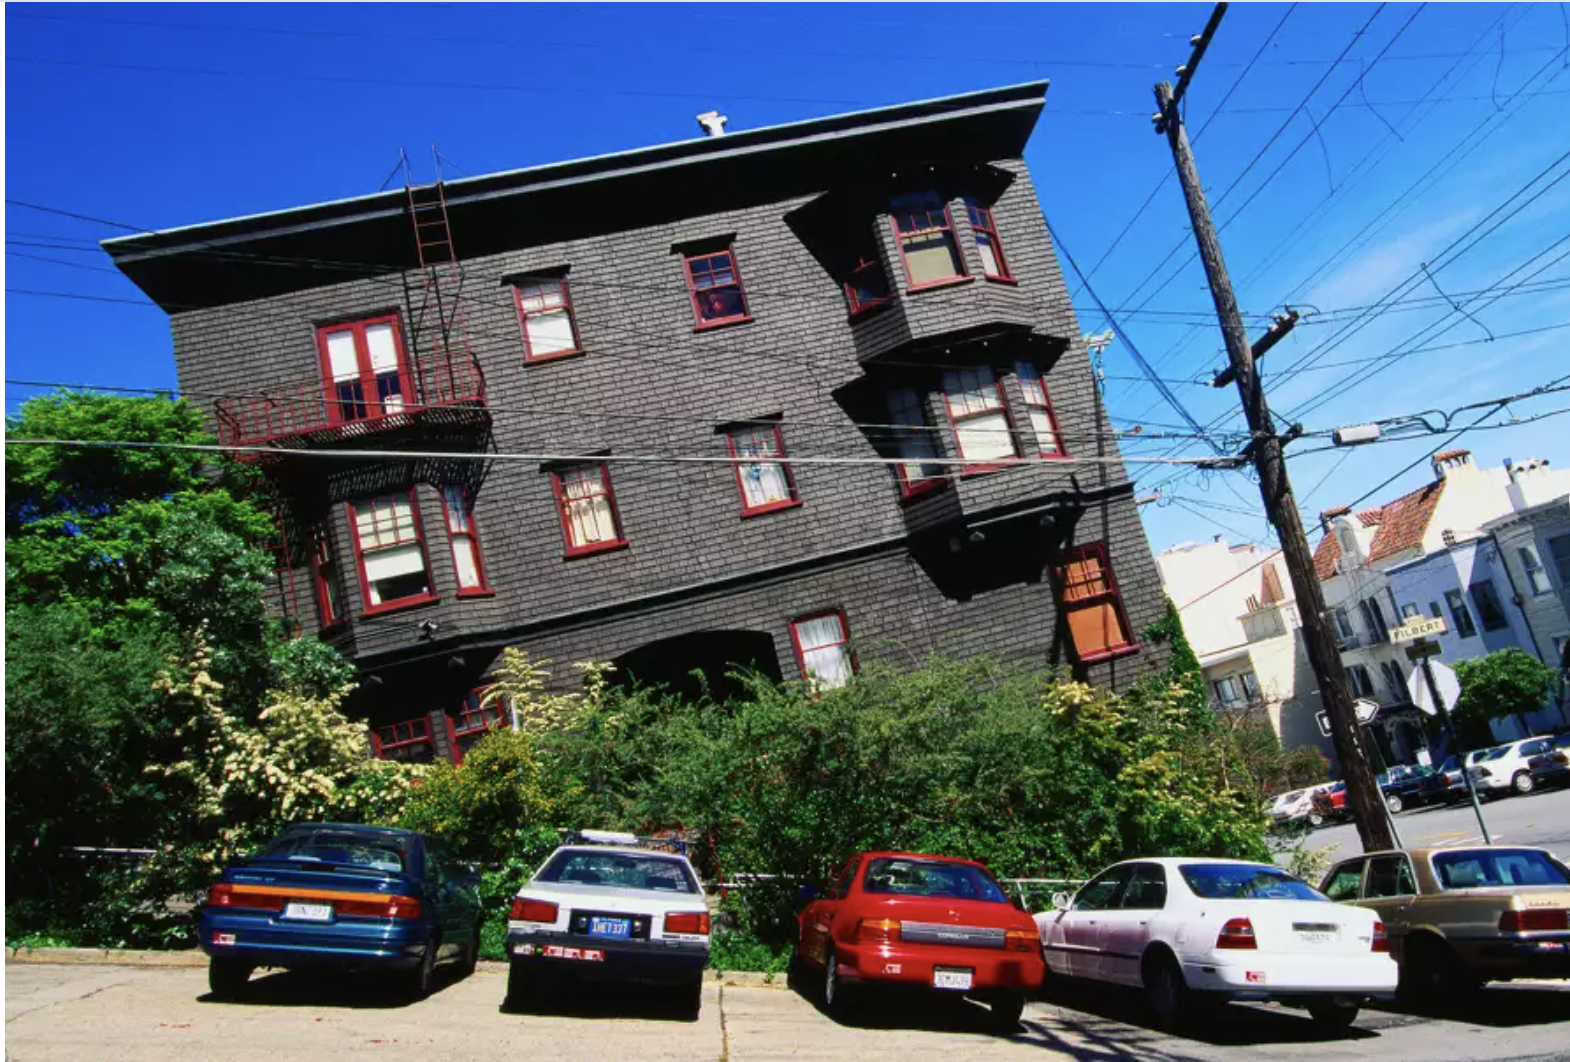
\includegraphics[width=\linewidth]{images/san_fran.png}}
\onslide<2->{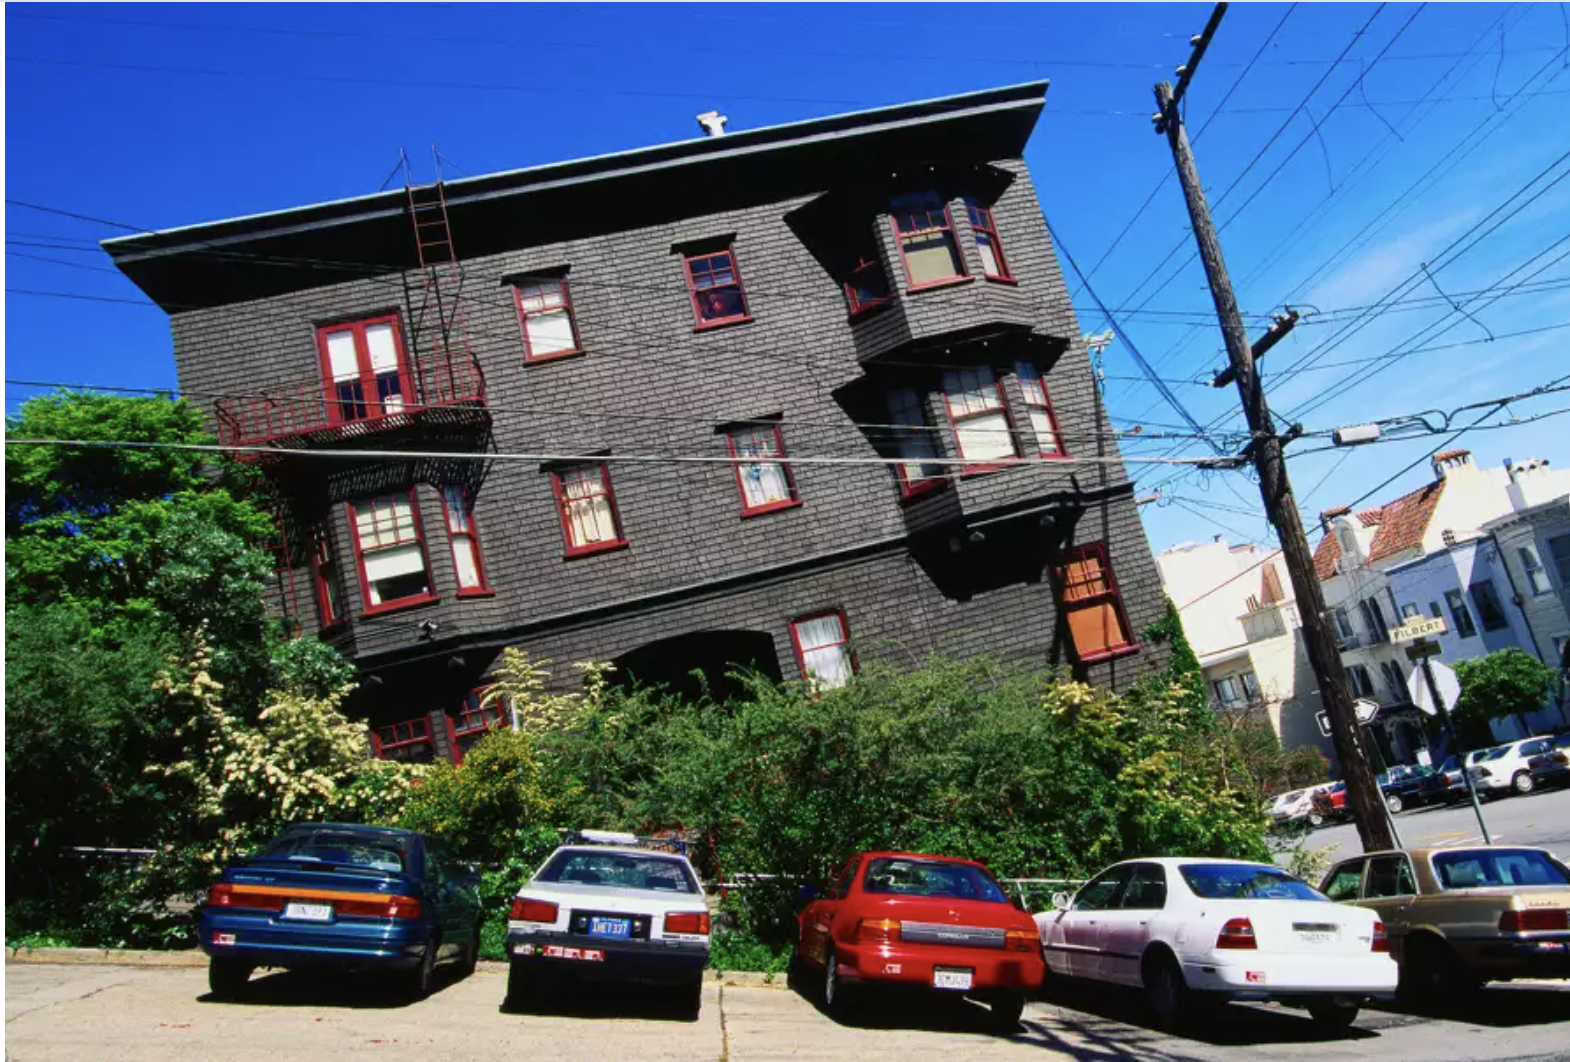
\includegraphics[width=\linewidth]{images/san_fran.png}\\[1pt]{\scriptsize You live in S.F.}}

\vspace{0.3cm}
\onslide<9->{%
\tikzset{
  cnode/.style = {latent, minimum size=0.9cm, line width=1.0pt, font=\large},
  cedge/.style = {->, >=latex, line width=1.0pt},
}
\resizebox{0.5\linewidth}{!}{%
  \begin{tikzpicture}
    \node[cnode] (x) at (-1, 0)  {$E$};
    \node[cnode] (y) at ( 1, 0)  {$B$};
    %\node[cnode] (z) at ( 0,-2)    {$C$};
    \alt<10>{\node[cnode, fill=gray!40] (z) at ( 0,-2) {$C$};}{\node[cnode] (z) at ( 0,-2) {$C$};}
    \draw[cedge] (x) -- (z);
    \draw[cedge] (y) -- (z);
  \end{tikzpicture}%
  }}
\end{column}
\end{columns}

\vfill
\only<8>{
\colorbox{red!30}{\textbf{Terminology.}} $E$ and $B$ are \textbf{marginally} independent but \textbf{conditionally} dependent (given $C$).
}

\only<9->{
\colorbox{yellow!30}{\textbf{Graphical View.}} The graph is drawn above.  $E$ and $B$ are independent unless we observe $C$.
}


\end{frame}





\begin{frame}{Three Canonical Graphs}

\only<1-4>{
\begin{figure}
\centering
% shared look for the three canonical graphs
\tikzset{
  cnode/.style = {latent, minimum size=1.1cm, line width=1pt, font=\Large},
  cedge/.style = {->, >=latex, line width=1pt},
}
\resizebox{0.9\textwidth}{!}{%
\begin{subfigure}[b]{0.31\textwidth}
  \centering
  \begin{tikzpicture}
    \node[cnode] (z) at ( 0, 0)    {$Z$};
    \node[cnode] (x) at (-1,-2)  {$X$};
    \node[cnode] (y) at ( 1,-2)  {$Y$};
    \draw[cedge] (z) -- (x);
    \draw[cedge] (z) -- (y);
  \end{tikzpicture}
  \caption{Fork} 
\end{subfigure}
\hfill \pause
\begin{subfigure}[b]{0.31\textwidth}
  \centering
  \begin{tikzpicture}
    \node[cnode] (x) at (-1, 0)  {$X$};
    \node[cnode] (y) at ( 1, 0)  {$Y$};
    \node[cnode] (z) at ( 0,-2)    {$Z$};
    \draw[cedge] (x) -- (z);
    \draw[cedge] (y) -- (z);
  \end{tikzpicture}
  \caption{Collider}
\end{subfigure}
\hfill \pause 
\begin{subfigure}[b]{0.31\textwidth}
  \centering
  \begin{tikzpicture}
    \node[cnode] (x) at (0, 0)  {$X$};
    \node[cnode] (z) at (0,-2)  {$Z$};
    \node[cnode] (y) at (0,-4)  {$Y$};
    \draw[cedge] (x) -- (z);
    \draw[cedge] (z) -- (y);
  \end{tikzpicture}
  \caption{Chain}
\end{subfigure}
}
\caption{\textbf{Three canonical graphs}}
\label{fig:three_canonical_graphs}
\end{figure}
}


\only<5->{
\begin{figure}
\centering
% shared look for the three canonical graphs
\tikzset{
  cnode/.style = {latent, minimum size=1.1cm, line width=1pt, font=\Large},
  cedge/.style = {->, >=latex, line width=1pt},
}
\resizebox{0.9\textwidth}{!}{%
\begin{subfigure}[b]{0.31\textwidth}
  \centering
  \begin{tikzpicture}
    \node[cnode, fill=gray!30] (z) at ( 0, 0)    {$Z$};
    \node[cnode] (x) at (-1,-2)  {$X$};
    \node[cnode] (y) at ( 1,-2)  {$Y$};
    \draw[cedge] (z) -- (x);
    \draw[cedge] (z) -- (y);
  \end{tikzpicture}
  \caption{Fork}
\end{subfigure}
\hfill 
\begin{subfigure}[b]{0.31\textwidth}
  \centering
  \begin{tikzpicture}
    \node[cnode] (x) at (-1, 0)  {$X$};
    \node[cnode] (y) at ( 1, 0)  {$Y$};
    \node[cnode] (z) at ( 0,-2)    {$Z$};
    \draw[cedge] (x) -- (z);
    \draw[cedge] (y) -- (z);
  \end{tikzpicture}
  \caption{Collider}
\end{subfigure}
\hfill 
\begin{subfigure}[b]{0.31\textwidth}
  \centering
  \begin{tikzpicture}
    \node[cnode] (x) at (0, 0)  {$X$};
    \node[cnode, fill=gray!30] (z) at (0,-2)  {$Z$};
    \node[cnode] (y) at (0,-4)  {$Y$};
    \draw[cedge] (x) -- (z);
    \draw[cedge] (z) -- (y);
  \end{tikzpicture}
  \caption{Chain}
\end{subfigure}
\hfill
}
\caption{\textbf{Three canonical graphs}}
\label{fig:three_canonical_graphs}
\end{figure}
}


\only<4-7>{\colorbox{yellow!30}{\textbf{Poll.}} When is $X$ independent of $Y$?}
%
\only<5-7>{\colorbox{green!30}{\textbf{Solution.}}  \only<5-7>{(a) If $Z$ is observed.}  \only<6-7>{(b)  If $Z$ (and all of its descendants) are \textbf{not} observed.}  \only<7>{(c) If $Z$ is observed.}}

\only<8>{\colorbox{green!30}{\textbf{The Big Idea.}} We can reason about independence in complicated probabilistic models by analyzing how paths between variables traverse through these three canonical graphs.}

\only<9-10>{\small \colorbox{red!30}{\textbf{Who Cares?}}}\only<10>{\small \; Finding independencies can make computations easier (see Group Exercise 1d from expectation and variance) and algorithms more scalable.}

\end{frame}




%\begin{frame}{Independence in Probabilistic Graphical Models: Example}
%\small
%
%A \textbf{Bayesian network} is a directed graph whose vertices are random events, and whose edges encode \textbf{dependence}.
%
%\vfill
%\begin{columns}[c,onlytextwidth]
%\begin{column}{0.39\textwidth}
%\centering
%\begin{tikzpicture}[
%    var/.style={rectangle, rounded corners=3pt, draw, thick, fill=blue!12, minimum height=7mm, align=center, font=\small},
%    >=latex, every edge/.style={draw, thick, ->}]
%  \node[var] (S) at (0,2.4) {Smoker ($S$)};
%  \node[var] (C) at (0,1.2) {Lung cancer ($C$)};
%  \node[var] (K) at (-1.15,0) {Cough ($K$)};
%  \node[var] (X) at (1.15,0) {Abnormal\\X-ray ($X$)};
%  \path (S) edge (C) (C) edge (K) (C) edge (X);
%\end{tikzpicture}
%\end{column}
%\begin{column}{0.58\textwidth}
%\footnotesize
%\begin{itemize}
%\item<1-> \textbf{An edge means direct dependence.}  Smoking changes the chance of cancer: $P(C \mid S) \neq P(C)$.
%\item<1-> \textbf{No edge doesn't mean independent.}  Smoker and Cough are dependent (smokers cough more), but only \textit{through} Lung cancer.
%\item<2-> \textbf{Common parent.}  Cough and X-ray are dependent (via cancer), but independent once we know about cancer. \only<3->{\alert{This is a fork.}}
%\item<4-> \textbf{Conditional independence.}  Once we know whether someone has cancer, smoking tells us nothing more about the cough: $P(K \mid C, S) = P(K \mid C)$. \only<5->{\alert{This is a chain.}}
%\end{itemize}
%\end{column}
%\end{columns}
%
%\vfill
%\onslide<1->{\colorbox{yellow!30}{\textbf{Factorization.}} $P(S, C, K, X) = P(S)\, P(C \mid S)\, P(K \mid C)\, P(X \mid C)$}
%\end{frame}
%
%






\begin{frame}[standout]
Group exercises
\end{frame}

\begin{frame}{Random group assignments}
%%% TABLE 1: by last name
\begin{columns}
\begin{column}{0.33\textwidth}
Ashley, Isabelle: 9 \\ 
Bailey, Tanna: 5 \\ 
Blaisdell, Olyver: 10 \\ 
Brown, Ashton: 11 \\ 
Cardenas, Dominic: 8 \\ 
Cutler, George: 12 \\ 
Fabik, Roland: 9 \\ 
Fellows, Audrey: 10 \\ 
Fitzgerald, Ryan: 11 \\ 
Fuller, Ryan: 3 \\ 
Griffen, Clara: 2 \\ 
Grutsch, Tanner: 3 \\\end{column}
\begin{column}{0.33\textwidth}
Hager, Nathan: 6 \\ 
Horner, Jayden: 4 \\ 
Johnson, Jaret: 5 \\ 
Kintzel, Samantha: 1 \\ 
Lameres, Alexis: 6 \\ 
Lee, Holden: 12 \\ 
Mayala, Reece: 4 \\ 
McLean, Connor: 11 \\ 
Mcbride, Daniel: 10 \\ 
Miller, Maverick: 7 \\ 
Moss, Emily: 8 \\ 
Mousseau, Matthew: 8 \\\end{column}
\begin{column}{0.33\textwidth}
Neuman, Evan: 12 \\ 
Putnam, John: 1 \\ 
Ramos, Vydel: 3 \\ 
Rathbun, Jedidiah: 7 \\ 
Roberts, Matthew: 7 \\ 
Roller, Nathan: 2 \\ 
Ryan, Otis: 4 \\ 
Shevtsov, Timothy: 6 \\ 
Stensland, Emma: 1 \\ 
Thiessen, Logan: 5 \\ 
Thompson, Jaiden: 9 \\ 
Vath, Ethan: 2 \\\end{column}
\end{columns}
\end{frame}

\begin{frame}{Group exercises}
\small 
\noindent
\begin{minipage}[c]{0.6\textwidth}
\begin{enumerate}
	\item  Write the graph in the top figure as a pair of sets $(V, E)$.
	\item Draw a picture of the graph below
	  \resizebox{\linewidth}{!}{$
	   \bigg( \set{a,b,c,d,e}, \; \bigg\{  \set{a,b}, \set{a,c}, \set{a,d}, \set{b,e}, \set{c,d} \bigg\} \bigg) 	
	$.}
    \item Construct a graph for which the is-adjacent relation, $\sim$, is transitive.
    \item How many edges are in $K_n$, a complete graph with $n$ vertices?
    \item How many different graphs can be formed with vertex set $V=\set{1,2,3,\hdots,n}$?
    \item Prove that in every graph, the number of vertices with odd degree is even. (For example, the graph from the reading quiz, reproduced in the bottom figure, has exactly four vertices of odd degree.)
\end{enumerate}
\end{minipage}%
\hfill
\begin{minipage}[c]{0.38\textwidth}
    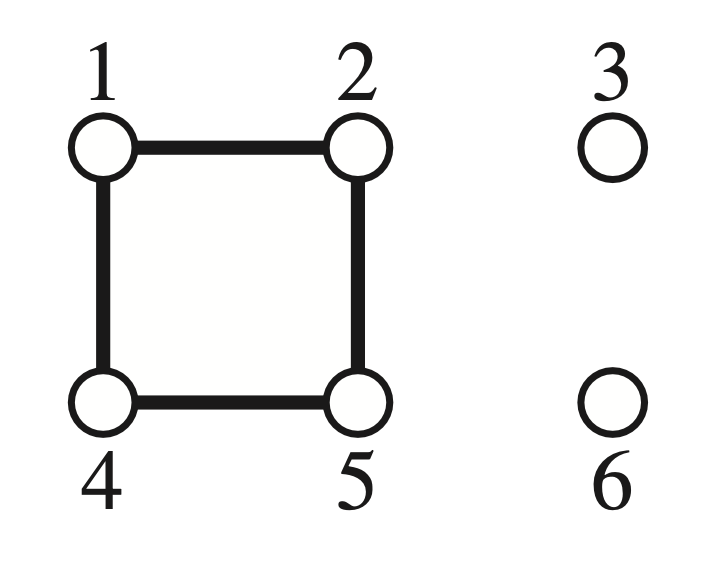
\includegraphics[width=\textwidth]{images/simple_graph_2} %
    \vfill 
    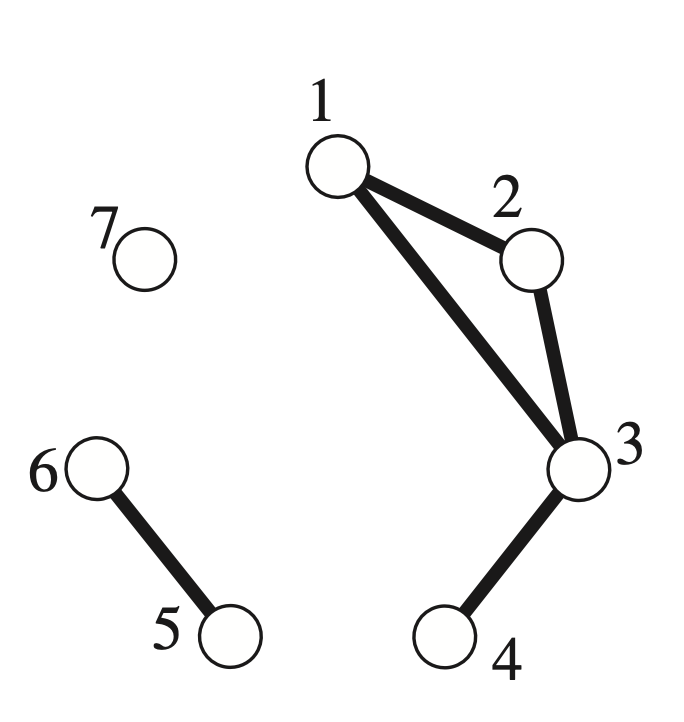
\includegraphics[width=\textwidth]{images/simple_graph.png}
\end{minipage}%    

\end{frame}




\begin{frame}{Solution to group exercise \#1}
\small 
\textbf{Problem.} Write the graph below as a pair of sets $(V, E)$.
\vfill 
\begin{center}
    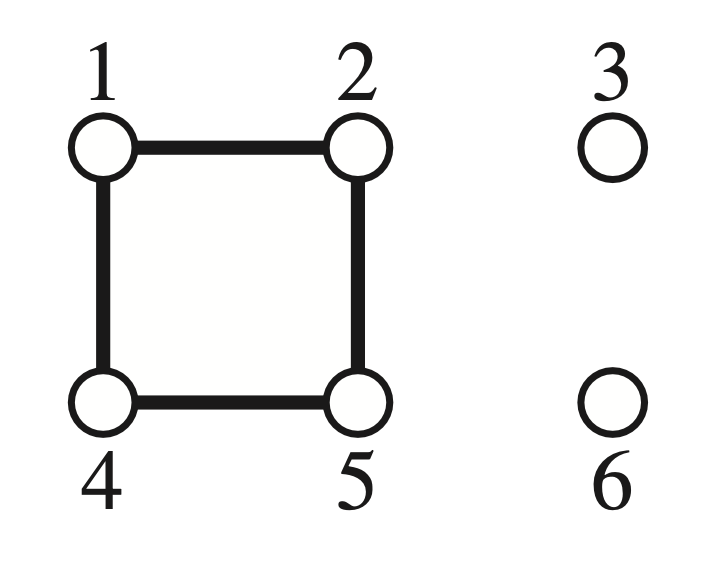
\includegraphics[width=.5\textwidth]{images/simple_graph_2} %
\end{center}   

\vfill 

\textbf{Solution.}
\[ \bigg( \set{1,2,3,4,5,6}, \bigg\{ \set{1,2}, \set{2,5}, \set{5,4}, \set{1,4} \bigg\} \bigg) \]
    
\end{frame}



\begin{frame}{Solution to group exercise \#2}
\small 
\textbf{Problem.} Draw a picture of the graph below
	  \resizebox{\linewidth}{!}{$
	   \bigg( \set{a,b,c,d,e}, \; \bigg\{  \set{a,b}, \set{a,c}, \set{a,d}, \set{b,e}, \set{c,d} \bigg\} \bigg) 	
	$.}

\vfill 

\textbf{Solution.} There are many possible solutions.  For example:

\begin{center}
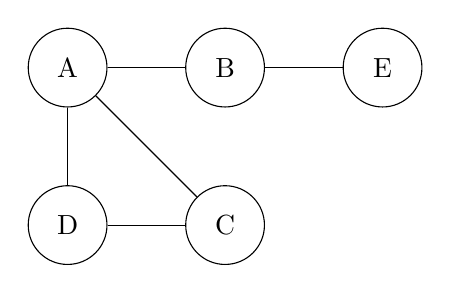
\begin{tikzpicture}[every node/.style={circle, draw, minimum size=1cm}, node distance=2cm]
    \node (A) {A};
    \node (B) [right of=A] {B};
    \node (C) [below of=B] {C};
    \node (D) [left of=C] {D};
    \node (E) [right of=B] {E};

    % Edges
    \draw (A) -- (B);
    \draw (A) -- (C);
    \draw (A) -- (D);
    \draw (B) -- (E);
    \draw (C) -- (D);
\end{tikzpicture}

\end{center}
\end{frame}


\begin{frame}{Solution to group exercise \#3}
\small 
\textbf{Problem.} Construct a graph for which the is-adjacent relation, $\sim$, is transitive.

\vfill 

\textbf{Solution.} There are many possible solutions.  For example:

\begin{minipage}{0.3\textwidth}
\vspace{.2cm}
\centering
This \\[1ex]
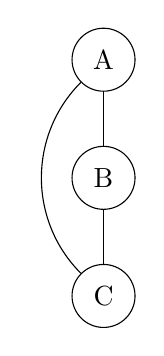
\begin{tikzpicture}[every node/.style={circle, draw, minimum size=0.8cm}, node distance=1.5cm]
    \node (A) {A};
    \node (B) [below of=A] {B};
    \node (C) [below of=B] {C};

    \draw (A) -- (B);
    \draw (B) -- (C);
    \draw (A) to[bend right=45]  (C);
\end{tikzpicture}
\end{minipage}
\hfill
\begin{minipage}{0.3\textwidth}
Or this \\[1ex]
\vspace{.2cm}
\centering
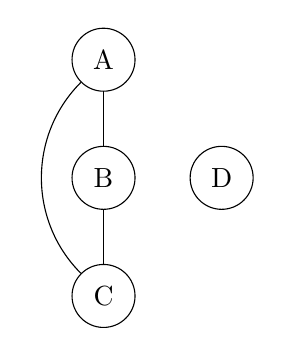
\begin{tikzpicture}[every node/.style={circle, draw, minimum size=0.8cm}, node distance=1.5cm]
    \node (A) {A};
    \node (B) [below of=A] {B};
    \node (C) [below of=B] {C};
    \node (D) [right of=B] {D};

    \draw (A) -- (B);
    \draw (B) -- (C);
    \draw (A) to[bend right=45]  (C);
\end{tikzpicture}
\end{minipage}
\hfill
\begin{minipage}{0.3\textwidth}
But not this \\[1ex]
\centering
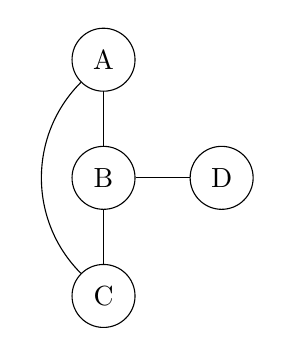
\begin{tikzpicture}[every node/.style={circle, draw, minimum size=0.8cm}, node distance=1.5cm]
    \node (A) {A};
    \node (B) [below of=A] {B};
    \node (C) [below of=B] {C};
    \node (D) [right of=B] {D};

    \draw (A) -- (B);
    \draw (B) -- (C);
    \draw (A) to[bend right=45]  (C);
    \draw (B) -- (D);
\end{tikzpicture}
\end{minipage}

\end{frame}


\begin{frame}{Solution to group exercise \#4}
\footnotesize 
\textbf{Problem.} How many edges are in $K_n$, a complete graph with $n$ vertices?

\vfill 
\begin{minipage}{0.4\textwidth}
\textbf{Example.} $K_5$ is shown to the right.
\end{minipage} %
\hfill
\begin{minipage}{0.55\textwidth}
\begin{figure}
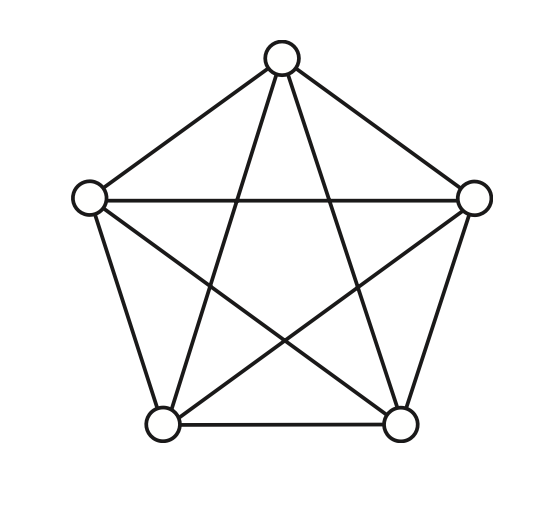
\includegraphics[width=.3\linewidth]{images/complete_graph.png}	
\end{figure}
\end{minipage} 

\vfill 

\textbf{Solution.} In a complete graph, all pairs of vertices are adjacent.  Since there are $\binom{n}{2} = \frac{n(n-1)}{2}$ ways to choose pairs of $n$ vertices, there must be $\binom{n}{2} = \frac{n(n-1)}{2}$ edges.

\vfill 

\textbf{Alternate Solution (From A Student).} We can use Theorem 47.5, which says
%
\begin{align}
\sum_{v \in V} d(v) = 2 |E|. 
\label{eqn:sum_of_degrees_gives_twice_the_edges}
\end{align}

In a complete graph, $d(v) = n-1$ for all vertices $v \in V$, since each vertex must be adjacent to all other vertices. Since there are $n$ vertices all together, we have

\[ \sum_{v \in V} d(v) =  n(n-1)  \]

Substituting this into \Eqref{eqn:sum_of_degrees_gives_twice_the_edges} and solving for $|E|$ yields the solution:
\[ |E| =   \frac{n(n-1)}{2}.\]


\end{frame}


\begin{frame}{Solution to group exercise \#5}
\small 
\textbf{Problem.} How many different graphs can be formed with vertex set $V=\set{1,2,3,\hdots,n}$?
\vfill 
%There are $2^{\binom{n}{2}}$ different graphs that can be formed from $n$ vertices.
\textbf{Solution.}  $2^{\raisebox{0.3ex}{\scriptsize$\binom{n}{2}$}}$.   To justify this, note:
\begin{itemize}
\item When forming a graph from $n$ vertices, there are $\binom{n}{2}=\frac{n(n-1)}{2}$ \underline{candidate} edges (since there are $\binom{n}{2}$ ways to choose pairs from a set of $n$ items).
\item  For each edge, we make a binary decision to include or exclude the edge in the graph.
\item  Thus, by the multiplication principle (and specifically Scheinerman Theorem 8.6), there are $2^{\raisebox{0.3ex}{\scriptsize$\binom{n}{2}$}}$ possible graphs that can be formed.  [Imagine forming a list of length $\binom{n}{2}$, where each entry in the list takes on one of 2 values (e.g. \texttt{include} or \texttt{exclude}) corresponding to whether that particular edge is included or excluded in the graph.]
\end{itemize}

	
\end{frame}

\begin{frame}{Solution to group exercise \#6 (Slide 1/2)} 
\footnotesize 
\textbf{Problem.} Prove that in every graph, the number of vertices with odd degree is even. 

\vfill 
\textbf{Remark.} If you'd like some motivation for this problem, check out Section 7.1 (pp.125-129) of \href{https://file.fouladi.ir/courses/discmath/books/Springer.Verlag.Discrete.Mathematics.Elementary.and.Beyond.ebook-TLFeBOOK.pdf}{\underline{\textcolor{blue}{the book by L\'aszl\'o Lov\'asz and others}}}.  It's a really fun read!

\vfill 

\textbf{Solution} (by L\'aszl\'o Lov\'asz).  One way of proving the theorem is to build up the graph one edge at a time, and observe how the parities of the degrees change. An example is shown in Figure 7.4. We start with a graph with no edge, in which every degree is 0, and so the number of nodes with odd degree is 0, which is an even number.
 
\begin{figure}
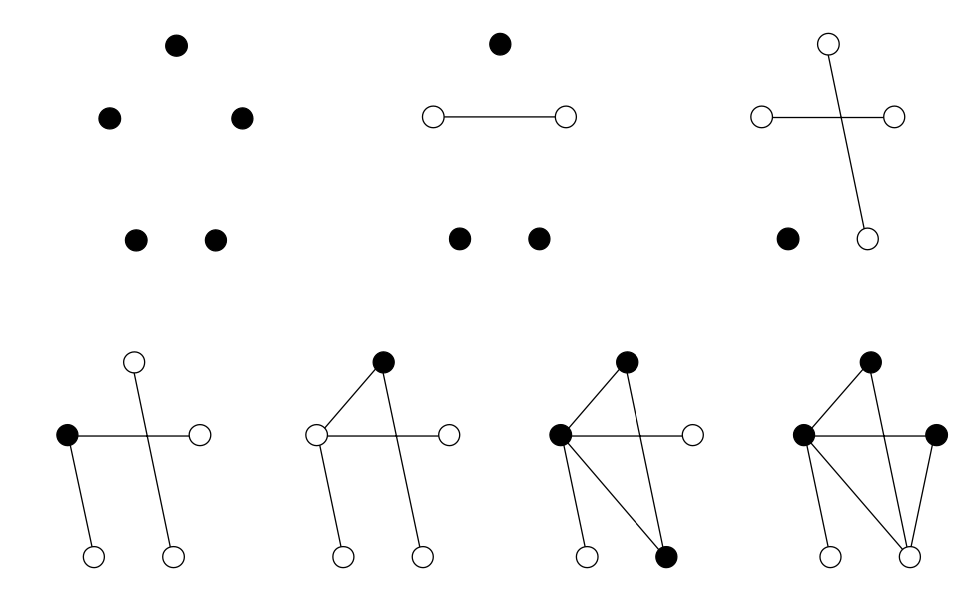
\includegraphics[width=.4\linewidth]{images/number_of_nodes_with_odd_degree_is_even.png}	
\caption{Building up a graph one edge at a time. Black circles mark nodes of even degree.}
\end{figure}

\hfill (See next slide for more.)

\end{frame}


\begin{frame}{Solution to group exercise \#6 (Slide 2/2)} 
\footnotesize 

\begin{figure}
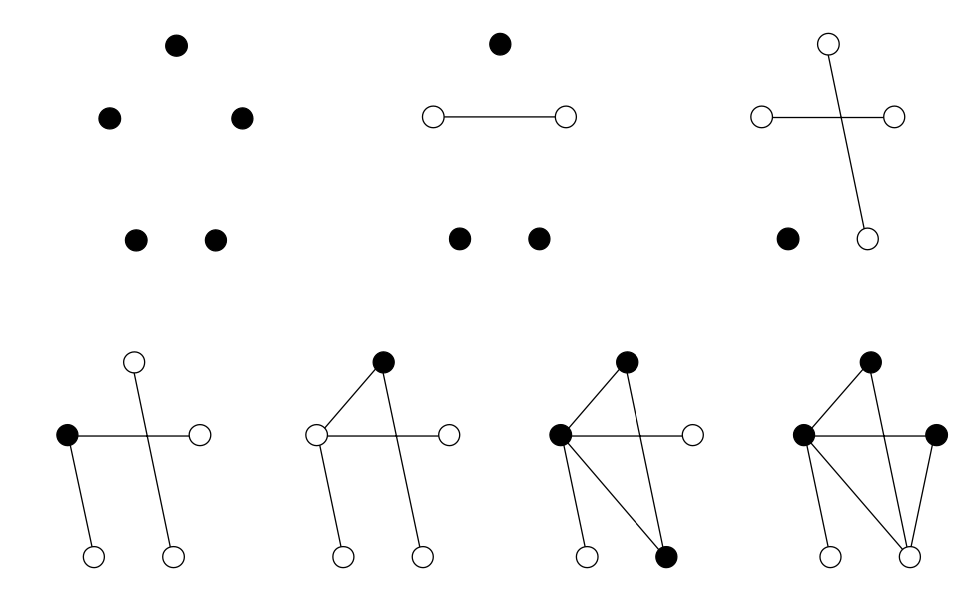
\includegraphics[width=.4\linewidth]{images/number_of_nodes_with_odd_degree_is_even.png}	
\end{figure}

\vspace{-.2cm}

Now if we connect two nodes by a new edge, we change the parity of the degrees at these nodes. In particular,
\begin{itemize}
\item if both endpoints of the new edge had even degree, we increase the number of nodes with odd degree by 2;
\item if both endpoints of the new edge had odd degree, we decrease the number of nodes with odd degree by 2;
\item if one endpoint of the new edge had even degree and the other had odd degree, then we don’t change the number of nodes with odd degree.
\end{itemize}

Thus if the number of nodes with odd degree was even before adding the new edge, it remained even after this step. This proves the theorem. (Note that this is a proof by induction on the number of edges.)

\end{frame}


\begin{frame}[standout]
Appendix	
\end{frame}



\begin{frame}{Probabilistic Graphical Models: General case}

\only<1->{
\begin{definition}
A \textit{Bayesian network} (also known as a belief network) is a representation of a joint probability distribution that specifies the conditional dependencies among random variables via a directed acyclic graph (DAG).
\end{definition}
}

\onslide<2->{
Let us represent the joint density of our model as follows:

\begin{align}
 p(x_1, ..., x_n) = \ds\prod_{i=1}^n p(x_i \cond \parents_i )
\label{eqn:joint_factorization_for_bayes_net} 
\end{align}
where $\parents_i$ refers to random variable $i$'s conditioning set, which is called the \textit{parents} of node $i$.
}
 

\only<3>{
Equation \eqref{eqn:joint_factorization_for_bayes_net} simplifies the factorization which is \textit{always} true, by the chain rule of probability:

\[ p(x_1, ..., x_n) = \ds\prod_{i=1}^n p(x_i \cond x_1, .., x_{i-1} ) \]
}

\only<4->{
We represent our model in \Eqref{eqn:joint_factorization_for_bayes_net} as a DAG by  
 identifying each random variable with a node, and drawing a directed edge from $X_j$ to $X_i$ if $X_j$ is a parent of $X_i$.
 } 
\end{frame}

\end{document}
